\section{Methods}
% https://www.scribbr.com/dissertation/methodology/
% https://www.youtube.com/watch?v=2MqLFH7CalQ
%
% It should include:
%
% The type of research you conducted
% How you collected and analyzed your data
% Any tools or materials you used in the research
% How you mitigated or avoided research biases
% Why you chose these methods
%
% Your methodology section should generally be written in the PAST TENSE!
\begin{comment}
In our work on text classification, it was important to directly measure how changes in our methodological factors (independent variables) influenced performance metrics (dependent variables). Our primary focus was to assess the relative effectiveness of different models among machine learning and large language models -- long short-term memory, non-reasoning and reasoning-enabled LLMs -- in classifying unstructured text data. Chosing a controlled experiment letted us tweak one or more factors (for example, feature extraction or model parameters) while keeping all other conditions the same. This controlled setting made it easier to observe and measure the impact on key performance indicators, like classification accuracy or F1-score, using statistical tests. The collection of numerical measurements from our experiments inherently made our approach quantitative.

Wohlin et al. \cite{wohlin2000software} explain that controlled experiments provide a clear way to investigate cause-and-effect relationships. Compared to surveys or case studies -- which may mix in effects from uncontrolled factors -- a controlled experiment minimizes external influences. This allows us to be more confident that any changes in the performance of our text classification system are due to the specific modifications we introduced rather than random variation.
\end{comment}

Based on our focus on text classification, this thesis aims to address several core questions (RQ1 to RQ4). Our first three research questions concern accuracy (RQ1), cost and time efficiency (RQ2), and applicability to hierarchical categorization (RQ3) for LSTM networks, LLMs without explicit reasoning, and LLMs with reasoning capabilities. To tackle these questions, we chose a controlled experiment: by systematically varying specific factors -- like feature extraction methods or model hyperparameters -- while keeping all other conditions the same, we can better isolate and measure the effects on performance metrics such as accuracy and F1-score \cite{wohlin2000software}. This experimental setup provides the quantitative structure necessary to compare the different models in a fair and transparent way, reducing the chances that outside influences distort our results.

Although RQ4 involves a case study with actual work orders, the basic methodology remains grounded in comparing the most promising models from the earlier steps. Thus, after completing our controlled experiments to identify which models excel in RQ1 through RQ3, we have proceeded with a practical application in RQ4. This final step allowed us to test relevance in an applied case by deploying the top-performing classifier in a multi-level categorization scenario resembling a professional setting relevant to UPTILT.

\subsection{Data collection}
% Step 2:
% Methods of data collection:
%
% - The sampling method or critera
% - The tools, procedures, and materials
% - How variables were measured

\begin{comment}
With our collaboration we got access to an extensive dataset consisting of anonymized Work Orders (WOs) derived from genuine service business operations. Each WO represented unstructured textual information described earlier in the Background section, including task descriptions, instructions, lists of materials, and other relevant details without structured formatting.

Before starting the iterations of the experiment, we further cleaned the dataset and removed any sensitive information. A method such as tokenization and word segmentation was applied using natural language toolkit (NLTK) --- a standard toolkit found in Python and recommended by \cite{bird2009nlp}. This process involved breaking the text into tokens (words, punctuation marks, etc.) and accurately identifying word boundaries and was our first step in the process. Stop-word removal was applied using the same library, eliminating common words \textit{("the", "is", "at" and more...)} that does not contribute any significant meaning to the text when used in conjunction with ML and LLMs. The text was further cleaned from any punctuations and symbols.    
\end{comment}

In collaboration with UPTILT, we obtained access to a dataset comprising anonymized Work Orders (WOs). These WOs originated from real-world service business operations and contained unstructured textual data, including elements such as task descriptions, operational instructions, and material lists, all lacking a predefined structure.

\begin{figure}[h!]
    \centering
    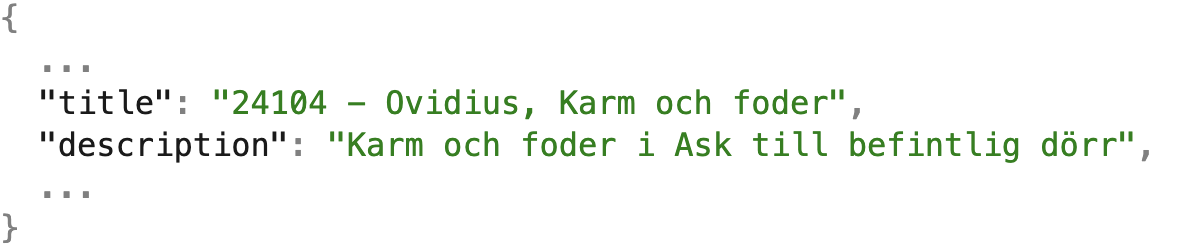
\includegraphics[width=1\linewidth]{img/fig4.png}
    \caption{Work order example}
    \label{fig:enter-label}
\end{figure}

Initially, we wanted to use this WO data to train machine learning models, specifically an support vector machine (SVM), to automatically classify them. However, we quickly realized this wouldn't work well. We couldn't get reliable 'ground truth' labels for the WOs, which are needed for training. This was because the data was already anonymized, historical, and we didn't have the resources to manually label thousands of them. On top of that, there simply wasn't enough WO data available to train an SVM model properly.

Because of these issues, we decided to change our approach. We kept the WO dataset, but instead of using it for the main machine learning experiments, we decided to use it for a detailed case study later in the project (this relates to our RQ4). This way, we could still learn from its real-world content.

For our main text classification experiments, we needed another dataset that did have labels and enough data. We chose the well-known "20 Newsgroups corpus" dataset \cite{Lang95}. We picked this one because the text in the newsgroup posts has some similarities to the WO text -- for example, it uses varied language and includes specific terms or abbreviations, making it complex in a similar way. Even though the topics are completely different, using this dataset allowed us to test our classification methods on text with similar kinds of challenges.

The 20 Newsgroups dataset, collected by Lang \cite{Lang95}, is commonly used in research for testing text classification. It contains about 20,000 documents from 20 different online news discussion groups. The documents are divided fairly evenly among the 20 groups, each covering a different topic. Some topics are closely related (like different computer groups), while others are very unrelated (like sales versus religion), which makes classifying the documents a good test for machine learning models.

\subsection{Data preparation}
To prepare this raw data for controlled experimentation and subsequent analysis, particularly for use with machine learning (ML) and large language models (LLMs), a dedicated data preprocessing pipeline was implemented using Python. This pipeline served to structure, clean, and normalize the textual content. The implementation primarily utilized the Pandas library for data manipulation and the Natural Language Toolkit (NLTK) \cite{bird2009nlp} for core text processing functionalities.

As a prerequisite, the pipeline ensured necessary NLTK resources were available by automatically downloading the 'stopwords' corpus, 'punkt' and the 'punkt\_tab' tokenizer models via the \verb|nltk.downloader| module.

The core data processing workflow involved the following key stages:

\begin{enumerate}
    \item \textbf{Loading and Structuring:} WO data were loaded from various JSON formats (files, strings, or objects) and structured into a tabular Pandas dataframe.
    \item \textbf{Selective Text Extraction:} Relevant textual content was selectively extracted from predefined fields (keys) within each record, focusing only on scalar values suitable for conversion to text.
    \item \textbf{Text Normalization:} Each extracted text segment was subjected to a standardized cleaning sequence: conversion to lowercase, removal of punctuation and symbols (retaining alphanumeric content), and filtering of common English stop words identified via NLTK.
    \item \textbf{Consolidation and Filtering:} The cleaned text segments from the relevant fields of each news article were concatenated into a single string. Records yielding an empty string after this process were subsequently removed.
\end{enumerate}

\begin{figure}[h!]
    \centering
    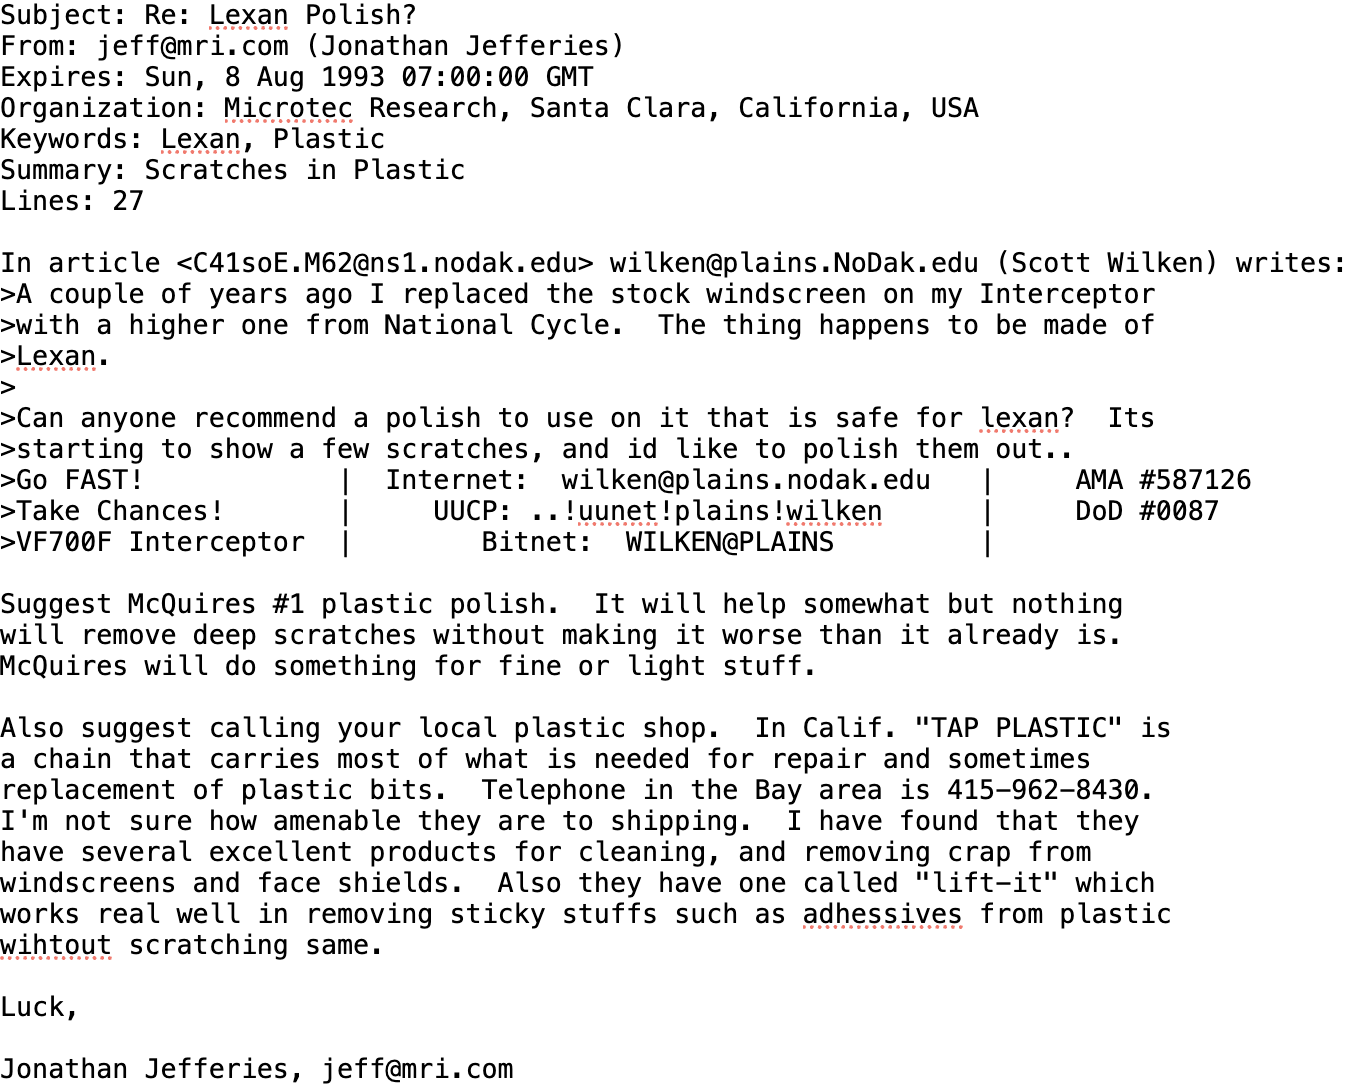
\includegraphics[width=0.8\linewidth]{img/fig2.png}
    \caption{Example of an unprocessed news article}
    \label{fig:enter-label}
\end{figure}

To facilitate a fair and reproducible comparison across multiple configurations, the dataset was then randomly divided using a fixed-seed splitting method rooted in digits of pi into two distinct subsets: training (~80\%) and testing (~20\%). The training set was used to train (or in the case of LLMs, prompt-engineer and fine-tune prompts for) classification models, while the testing dataset was reserved strictly for their performance evaluation.


\subsection{Experiment design}
% Continuing with design and setup subsection...
% As example:
% - The machine used
% - The software used (versions!)
% - What types of measurement tools where used (again versions, unless it is already a part of the software)
% Add sources/references here to support our choices!
% Specify the LLMs and ML models/algorithms used (e.g., GPT-4o, Deepseek, Naive Bayes).
%
% Explain why these models were chosen and how they are relevant to the research question.
% Describe whether the models are pre-trained, fine-tuned, or used with prompt engineering.
% Explain any hyperparameter tuning performed (e.g., learning rate, batch size).
% Discuss the computational resources required (e.g., GPUs, cloud services).
%
% Use references to support our choices here!
For our text classification task, we decided to compare two different types of models: Support Vector Machines (SVM), which is a well-known traditional machine learning algorithm, and Large Language Models (LLMs) like GPT, which represent newer deep learning methods.

Traditional methods like SVM have been used a lot for text classification in the past. They work by finding the best boundary to separate different categories of text. However, they usually need us to carefully create numerical features from the text first (like TF-IDF scores) and often require a good amount of labeled data to learn effectively. They might also struggle to fully capture the meaning that comes from the specific order of words in sentences \cite{sarker2021machine}.

We chose SVM as a strong baseline model for our experiments. SVMs are known to work well, especially when dealing with text data that has been converted into high-dimensional feature vectors \cite{Joachims1998}. Including SVM allows us to compare a solid, traditional classification method against the more recent LLM approach, giving us a clear benchmark.

In contrast, Large Language Models (LLMs), such as OpenAI's GPT-4 or Meta's LLaMA, are built using the Transformer architecture and are pre-trained on massive amounts of text. This pre-training gives them a broad understanding of language, allowing them to perform well on new tasks often with very little (few-shot) or sometimes even no (zero-shot) specific examples from our dataset \cite{brown2020language, touvron2023llama}. Studies consistently show that LLMs frequently outperform traditional ML models like SVMs on various text classification tasks \cite{moller2024parrot, betianu2024dallmi}. Fine-tuning an LLM can boost its accuracy even further. Another advantage is that LLMs can often work directly with text, reducing the need for complex data preprocessing and feature creation steps that SVMs require \cite{oh2024language}.

Therefore, our final selection was SVMs, representing a powerful classical approach that relies on feature representation, and GPT-based LLMs, representing the state-of-the-art in language understanding, known for their adaptability and few-shot learning capabilities. By comparing these two different methods -- a traditional feature-based classifier (SVM) versus a pre-trained, context-aware language model (LLM) -- we aim to answer our research questions (RQ1 and RQ2) about which approach works better for our specific text classification challenge.

\subsection{Variables}
A variable is anything that can change or be changed -- any factor that can be manipulated, controlled for, or measured in an experiment. In this study, we distinguish between two main types of variables: independent variables, which we manipulate to observe their effect, and dependent variables, which we measure to capture the outcomes.

Our independent variables include the choice of train and test subsets, the models and algorithms used, the specific model configurations, and the prompt. We hypothesize that each of these factors can directly influence the results. To assess their effects, we rely on our dependent variables, namely accuracy, precision, recall, and the F1-score. By measuring these metrics under various settings, we can compare and quantify how each independent variable impacts overall performance.

The four dependent variables is a combination of results from classifications.  A true positive (TP) means the predicted label matches the true label in contrast to the true negative (TN), which means the predicted label is "negative" and the actual label is also "negative." Both TPs and TNs represent accurate predictions, whereas a false positive (FP) or false negative (FN) indicates that the  classification was incorrect.

\medskip
Accuracy is the percentage of correct predictions over the total number of  predictions. More concretely, it measures how often the model labels samples  correctly compared to the total number of samples evaluated, and can be written  as: where $\mathrm{TP}$ is the number of true positives, $\mathrm{TN}$ is the  number of true negatives, $\mathrm{FP}$ is the number of false positives,  and $\mathrm{FN}$ is the number of false negatives.

$$
\mathrm{Accuracy} = \frac{\mathrm{TP} + \mathrm{TN}}
{\mathrm{TP} + \mathrm{TN} + \mathrm{FP} + \mathrm{FN}}
$$

\medskip
Precision displays the model’s accuracy in predicting a particular label (also known as class).  In other words, it measures how often the model is correct when it predicts that label. The sum was calculated as follows: where $\mathrm{TP}$ is the number of true positives and $\mathrm{FP}$ is the number of false positives.

$$
\mathrm{Precision} 
= \frac{\mathrm{TP}}{\mathrm{TP} + \mathrm{FP}}
$$

\medskip
Recall can be seen as the ratio of positively recognized samples to all samples  in the actual label -- $\mathrm{TP}$ and $\mathrm{FN}$, where $\mathrm{TP}$ denotes the number of true positives, and $\mathrm{FN}$ represents the number of false negatives.

$$
\mathrm{Recall} = \frac{\mathrm{TP}}{\mathrm{TP} + \mathrm{FN}}
$$

\medskip
F1 Score is the harmonic mean between Precision and Recall. More concretely, it is a single metric  that balances the trade-off between both metrics, especially useful when we need a combined measure.  Was calculated as follows: where $\mathrm{Precision}$ is the fraction of predicted positives that are  truly positive, and $\mathrm{Recall}$ is the fraction of actual positives that are predicted positive.

$$
\mathrm{F1} = \frac{2 \times \mathrm{Precision} \times \mathrm{Recall}}
{\mathrm{Precision} + \mathrm{Recall}}
$$

% --------------------------------------------

Since we did not have access to a domain expert from the specific service business area, prompt construction was based on available domain documentation and published industry terminology in similar fields. To ensure correctness and appropriateness, we systematically referred to standard terminology used in similar industry reports and publicly available domain-specific resources throughout the prompt development stage. Although involving a domain expert is highly recommended, our documentation of each iteration still provides reproducibility. However, the absence of expert validation remains a limitation of our approach.